% Options for packages loaded elsewhere
\PassOptionsToPackage{unicode}{hyperref}
\PassOptionsToPackage{hyphens}{url}
\documentclass[
]{article}
\usepackage{xcolor}
\usepackage[margin=1in]{geometry}
\usepackage{amsmath,amssymb}
\setcounter{secnumdepth}{-\maxdimen} % remove section numbering
\usepackage{iftex}
\ifPDFTeX
  \usepackage[T1]{fontenc}
  \usepackage[utf8]{inputenc}
  \usepackage{textcomp} % provide euro and other symbols
\else % if luatex or xetex
  \usepackage{unicode-math} % this also loads fontspec
  \defaultfontfeatures{Scale=MatchLowercase}
  \defaultfontfeatures[\rmfamily]{Ligatures=TeX,Scale=1}
\fi
\usepackage{lmodern}
\ifPDFTeX\else
  % xetex/luatex font selection
\fi
% Use upquote if available, for straight quotes in verbatim environments
\IfFileExists{upquote.sty}{\usepackage{upquote}}{}
\IfFileExists{microtype.sty}{% use microtype if available
  \usepackage[]{microtype}
  \UseMicrotypeSet[protrusion]{basicmath} % disable protrusion for tt fonts
}{}
\makeatletter
\@ifundefined{KOMAClassName}{% if non-KOMA class
  \IfFileExists{parskip.sty}{%
    \usepackage{parskip}
  }{% else
    \setlength{\parindent}{0pt}
    \setlength{\parskip}{6pt plus 2pt minus 1pt}}
}{% if KOMA class
  \KOMAoptions{parskip=half}}
\makeatother
\usepackage{color}
\usepackage{fancyvrb}
\newcommand{\VerbBar}{|}
\newcommand{\VERB}{\Verb[commandchars=\\\{\}]}
\DefineVerbatimEnvironment{Highlighting}{Verbatim}{commandchars=\\\{\}}
% Add ',fontsize=\small' for more characters per line
\usepackage{framed}
\definecolor{shadecolor}{RGB}{248,248,248}
\newenvironment{Shaded}{\begin{snugshade}}{\end{snugshade}}
\newcommand{\AlertTok}[1]{\textcolor[rgb]{0.94,0.16,0.16}{#1}}
\newcommand{\AnnotationTok}[1]{\textcolor[rgb]{0.56,0.35,0.01}{\textbf{\textit{#1}}}}
\newcommand{\AttributeTok}[1]{\textcolor[rgb]{0.13,0.29,0.53}{#1}}
\newcommand{\BaseNTok}[1]{\textcolor[rgb]{0.00,0.00,0.81}{#1}}
\newcommand{\BuiltInTok}[1]{#1}
\newcommand{\CharTok}[1]{\textcolor[rgb]{0.31,0.60,0.02}{#1}}
\newcommand{\CommentTok}[1]{\textcolor[rgb]{0.56,0.35,0.01}{\textit{#1}}}
\newcommand{\CommentVarTok}[1]{\textcolor[rgb]{0.56,0.35,0.01}{\textbf{\textit{#1}}}}
\newcommand{\ConstantTok}[1]{\textcolor[rgb]{0.56,0.35,0.01}{#1}}
\newcommand{\ControlFlowTok}[1]{\textcolor[rgb]{0.13,0.29,0.53}{\textbf{#1}}}
\newcommand{\DataTypeTok}[1]{\textcolor[rgb]{0.13,0.29,0.53}{#1}}
\newcommand{\DecValTok}[1]{\textcolor[rgb]{0.00,0.00,0.81}{#1}}
\newcommand{\DocumentationTok}[1]{\textcolor[rgb]{0.56,0.35,0.01}{\textbf{\textit{#1}}}}
\newcommand{\ErrorTok}[1]{\textcolor[rgb]{0.64,0.00,0.00}{\textbf{#1}}}
\newcommand{\ExtensionTok}[1]{#1}
\newcommand{\FloatTok}[1]{\textcolor[rgb]{0.00,0.00,0.81}{#1}}
\newcommand{\FunctionTok}[1]{\textcolor[rgb]{0.13,0.29,0.53}{\textbf{#1}}}
\newcommand{\ImportTok}[1]{#1}
\newcommand{\InformationTok}[1]{\textcolor[rgb]{0.56,0.35,0.01}{\textbf{\textit{#1}}}}
\newcommand{\KeywordTok}[1]{\textcolor[rgb]{0.13,0.29,0.53}{\textbf{#1}}}
\newcommand{\NormalTok}[1]{#1}
\newcommand{\OperatorTok}[1]{\textcolor[rgb]{0.81,0.36,0.00}{\textbf{#1}}}
\newcommand{\OtherTok}[1]{\textcolor[rgb]{0.56,0.35,0.01}{#1}}
\newcommand{\PreprocessorTok}[1]{\textcolor[rgb]{0.56,0.35,0.01}{\textit{#1}}}
\newcommand{\RegionMarkerTok}[1]{#1}
\newcommand{\SpecialCharTok}[1]{\textcolor[rgb]{0.81,0.36,0.00}{\textbf{#1}}}
\newcommand{\SpecialStringTok}[1]{\textcolor[rgb]{0.31,0.60,0.02}{#1}}
\newcommand{\StringTok}[1]{\textcolor[rgb]{0.31,0.60,0.02}{#1}}
\newcommand{\VariableTok}[1]{\textcolor[rgb]{0.00,0.00,0.00}{#1}}
\newcommand{\VerbatimStringTok}[1]{\textcolor[rgb]{0.31,0.60,0.02}{#1}}
\newcommand{\WarningTok}[1]{\textcolor[rgb]{0.56,0.35,0.01}{\textbf{\textit{#1}}}}
\usepackage{longtable,booktabs,array}
\usepackage{calc} % for calculating minipage widths
% Correct order of tables after \paragraph or \subparagraph
\usepackage{etoolbox}
\makeatletter
\patchcmd\longtable{\par}{\if@noskipsec\mbox{}\fi\par}{}{}
\makeatother
% Allow footnotes in longtable head/foot
\IfFileExists{footnotehyper.sty}{\usepackage{footnotehyper}}{\usepackage{footnote}}
\makesavenoteenv{longtable}
\usepackage{graphicx}
\makeatletter
\newsavebox\pandoc@box
\newcommand*\pandocbounded[1]{% scales image to fit in text height/width
  \sbox\pandoc@box{#1}%
  \Gscale@div\@tempa{\textheight}{\dimexpr\ht\pandoc@box+\dp\pandoc@box\relax}%
  \Gscale@div\@tempb{\linewidth}{\wd\pandoc@box}%
  \ifdim\@tempb\p@<\@tempa\p@\let\@tempa\@tempb\fi% select the smaller of both
  \ifdim\@tempa\p@<\p@\scalebox{\@tempa}{\usebox\pandoc@box}%
  \else\usebox{\pandoc@box}%
  \fi%
}
% Set default figure placement to htbp
\def\fps@figure{htbp}
\makeatother
\setlength{\emergencystretch}{3em} % prevent overfull lines
\providecommand{\tightlist}{%
  \setlength{\itemsep}{0pt}\setlength{\parskip}{0pt}}
\usepackage{hyperref}
\usepackage{amsmath}
\usepackage{amssymb}
\usepackage{graphicx}
\usepackage{fontspec}
\usepackage{xcolor}
\usepackage{tikz}
\definecolor{blue}{RGB}{0, 0, 100}
\setmainfont{Times New Roman}
\setsansfont{Times New Roman}
\setmonofont{Courier New}
\usepackage[margin=1in]{geometry}
\usepackage{titlesec}
\titleformat{\section}{\Huge\bfseries\color{blue}}{\thesection}{1em}{}
\titleformat{\subsection}{\huge\bfseries\color{blue}}{\thesubsection}{1em}{}
\titleformat{\subsubsection}{\LARGE\bfseries\color{blue}}{\thesubsubsection}{1em}{}
\usepackage{tocloft}
\renewcommand{\cftsecfont}{\small}
\renewcommand{\cftsubsecfont}{\footnotesize}
\renewcommand{\cftsecpagefont}{\small}
\renewcommand{\cftsubsecpagefont}{\footnotesize}
\renewcommand{\cftsecleader}{\cftdotfill{\cftdotsep}}
\usepackage{fontspec}
\usepackage{multirow}
\usepackage{multicol}
\usepackage{colortbl}
\usepackage{hhline}
\newlength\Oldarrayrulewidth
\newlength\Oldtabcolsep
\usepackage{longtable}
\usepackage{array}
\usepackage{hyperref}
\usepackage{float}
\usepackage{wrapfig}
\usepackage{bookmark}
\IfFileExists{xurl.sty}{\usepackage{xurl}}{} % add URL line breaks if available
\urlstyle{same}
\hypersetup{
  hidelinks,
  pdfcreator={LaTeX via pandoc}}

\author{}
\date{\vspace{-2.5em}}

\begin{document}

\begin{titlepage}
    \begin{center}
    % Début de la bordure avec TikZ
    \begin{tikzpicture}[remember picture, overlay] % overlay = force TikZ à dessiner par-dessus le contenu existant de la page, plutôt que de réserver un espace supplémentaire pour le dessin, remember = lorsque vous voulez dessiner par rapport à la position exacte de la page
    % Définir une couleur élégante
    \definecolor{blue}{RGB}{0, 100, 0}
    
    % Dessiner une bordure élégante avec coins arrondis
    \draw[
        line width=5pt, % Épaisseur du trait
        black, % Couleur de la bordure
        rounded corners=15pt, % Coins arrondis
        double, % Bordure double
        double distance=2pt % Espacement entre les deux lignes
    ] 
        ([xshift=10pt, yshift=-10pt]current page.north west) rectangle
        ([xshift=-10pt, yshift=10pt]current page.south east);
    \end{tikzpicture}
        
\includegraphics[width=7cm]{Figures/LOGO1.jpeg} \\[0.1cm]
        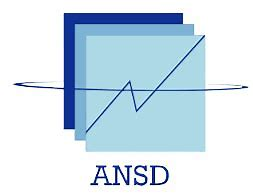
\includegraphics[width=6cm]{Figures/LOGO2.jpeg} \\[0.1cm]
        
        \textbf{\large Agence nationale de la Statistique et de la Démographie (ANSD)}\\[0.2cm]
        
        
\includegraphics[width=4cm]{Figures/LOGO3.jpeg} \\[0.1cm]
        
        \textbf{\large Ecole nationale de la Statistique et de l'Analyse économique Pierre Ndiaye (ENSAE)}\\[0.4cm]
        
        \textit{\LARGE Semestre 2 : Projet statistique sous R }\\[0.3cm]
        \textbf{\Huge \color{blue} \textsf{Partie 2 : Génération de rapports sur Word avec Rmarkdown}}\\[0.2cm]
        
        \begin{minipage}{0.5\textwidth}
    \begin{flushleft} \large
        \emph{\textsf{Rédigé par :}}\\
        \textbf{Khadidiatou Diakhaté}\\
        \textbf{Haba Fromo Francis}\\
        \textbf{Dior Mbengue}\\
    \end{flushleft}
\end{minipage}
        \hfill
        \begin{minipage}{0.4\textwidth}
            \begin{flushright} \large
                \emph{\textsf{Sous la supervision de :}} \\
                \textbf{M. Aboubacre HEMA}\\
                \textit{Research Analyst }
            \end{flushright}
        \end{minipage}

        \vfill 

        {\large \textsf{Année scolaire : 2024/2025}}\\[0.5cm]
        
    \end{center}
\end{titlepage}

\section{Introduction}\label{introduction}

La création de rapports statistiques professionnels nécessite des outils
adaptés pour produire des documents structurés, cohérents et
visuellement attrayants. RMarkdown s'est imposé comme une solution
incontournable pour les statisticiens et data scientists, permettant de
combiner du texte explicatif avec du code R exécutable et ses résultats
dans un même document.

\textbf{Pourquoi utiliser R Markdown pour générer un document Word ?}

\begin{itemize}
\item
  Automatisation de la rédaction : plus besoin de faire du copier-coller
  :
\item
  Séparation contenu / mise en forme : tu te concentres sur le fond, R
  s'occupe du rendu
\item
  Intégration directe de tableaux, graphiques, équations, bibliographies
\item
  Génération de rapports reproductibles, parfaits pour des livrables
  professionnels
\end{itemize}

Dans ce qui suit, nous explorons spécifiquement comment produire des
documents Word de qualité professionnelle avec RMarkdown. Bien que
RMarkdown offre plusieurs formats de sortie (HTML, PDF, etc.), le format
Word reste privilégié dans de nombreux contextes professionnels,
notamment dans les administrations et les organisations qui utilisent
principalement la suite Microsoft Office.

\subsection{Les packages officer, officedown, flextable, mschart,
rvg}\label{les-packages-officer-officedown-flextable-mschart-rvg}

Pour générer un document Word optimal avec RMarkdown, nous avons
délibérément choisi d'utiliser le package \textbf{officedown} avec le
template \textbf{Advanced Word Document} pour plusieurs raisons
essentielles :

\begin{enumerate}
\def\labelenumi{\arabic{enumi}.}
\item
  \textbf{Contrôle avancé de la mise en forme} : Contrairement au format
  Word standard de RMarkdown qui offre des options limitées, officedown
  permet un contrôle précis sur tous les aspects de mise en page
  (styles, en-têtes, pieds de page, colonnes multiples).
\item
  \textbf{Intégration avec l'écosystème R} : officedown s'intègre
  parfaitement avec les packages populaires comme flextable et mschart,
  offrant ainsi une expérience cohérente pour la présentation des
  tableaux et graphiques.
\item
  \textbf{Référencement croisé avancé} : Le template Advanced Word
  Document facilite la création et la gestion des références croisées
  entre figures, tableaux et sections.
\item
  \textbf{Compatibilité Microsoft Office} : Les documents générés sont
  pleinement compatibles avec les fonctionnalités de Microsoft Word,
  permettant une édition ultérieure sans perte de formatage.
\item
  \textbf{Environnement de travail unifié} : Ce template permet aux
  statisticiens de rester dans l'environnement R tout en produisant des
  documents qui répondent aux exigences des formats institutionnels.
\end{enumerate}

\subsection{Comment accéder au template Advanced Word Document
?}\label{comment-accuxe9der-au-template-advanced-word-document}

Pour accéder au template officedown et profiter de toutes ses
fonctionnalités, nous procédons comme suit :

\begin{enumerate}
\def\labelenumi{\arabic{enumi}.}
\tightlist
\item
  Dans RStudio, cliquez sur \textbf{File} \textgreater{} \textbf{New
  File} \textgreater{} \textbf{R Markdown}
\end{enumerate}

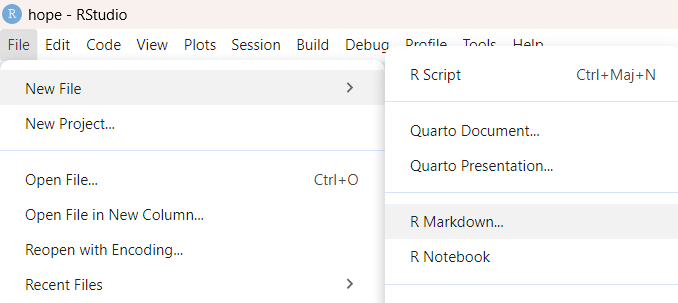
\includegraphics[width=4.67708in,height=\textheight,keepaspectratio]{images/clipboard-448743897.png}

\begin{enumerate}
\def\labelenumi{\arabic{enumi}.}
\setcounter{enumi}{1}
\tightlist
\item
  Dans la boîte de dialogue qui s'ouvre, sélectionnez l'onglet
  \textbf{From Template}, puis choisissez \textbf{Advanced Word
  document}
\end{enumerate}

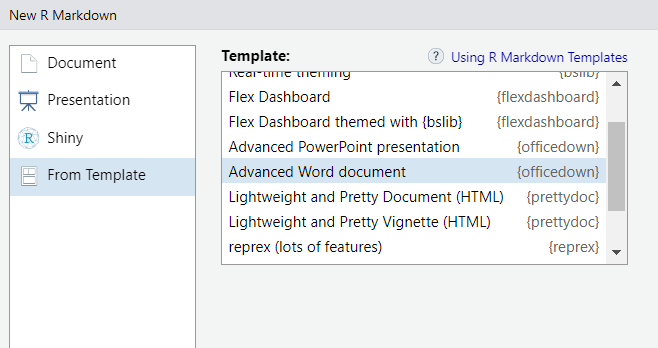
\includegraphics[width=4.67708in,height=\textheight,keepaspectratio]{images/clipboard-2214522613.png}

Cette sélection nous donne accès à un template enrichi spécifiquement
conçu pour la génération de documents Word professionnels. Explorons
maintenant comment l'utiliser efficacement et découvrons les
fonctionnalités avancées qu'il propose.

\section{I. Le YAML (Yet Another Markup
Language)}\label{i.-le-yaml-yet-another-markup-language}

Le YAML constitue l'en-tête du document RMarkdown et joue un rôle
crucial dans la configuration du document. Pour un document officedown,
la structure du YAML est particulièrement importante car elle détermine
comment le document sera transformé en format Word.

\subsection{Structure de base du YAML pour
officedown}\label{structure-de-base-du-yaml-pour-officedown}

\begin{Shaded}
\begin{Highlighting}[]
\PreprocessorTok{{-}{-}{-}}
\CommentTok{\# {-}{-}{-} MÉTADONNÉES DU DOCUMENT {-}{-}{-}}
\FunctionTok{date}\KeywordTok{:}\AttributeTok{ }\StringTok{"2025{-}04{-}18"}
\FunctionTok{author}\KeywordTok{:}\AttributeTok{ }\StringTok{"Votre Nom"}
\FunctionTok{title}\KeywordTok{:}\AttributeTok{ }\StringTok{"Titre du document"}

\CommentTok{\# {-}{-}{-} FORMAT DE SORTIE {-}{-}{-}}

\FunctionTok{output}\KeywordTok{:}\AttributeTok{ }
\AttributeTok{  officedown:}\FunctionTok{:rdocx\_document}\KeywordTok{:}\CommentTok{        \# Format de sortie Word via officedown}
\AttributeTok{    }\FunctionTok{reference\_docx}\KeywordTok{:}\AttributeTok{ }\StringTok{"template.docx"}\CommentTok{  \# Optionnel : utiliser un modèle Word existant}
\AttributeTok{    }\FunctionTok{mapstyles}\KeywordTok{:}\CommentTok{                       \# Permet d’associer des styles R Markdown à des styles Word}
\AttributeTok{      }\FunctionTok{Normal}\KeywordTok{:}\AttributeTok{ }\KeywordTok{[}\StringTok{\textquotesingle{}First Paragraph\textquotesingle{}}\KeywordTok{]}\CommentTok{    \# Le style "Normal" de R Markdown utilisera le style Word "First Paragraph"}
\AttributeTok{    }\FunctionTok{toc}\KeywordTok{:}\AttributeTok{ }\CharTok{true}\CommentTok{                         \# Table des matières}
\AttributeTok{    }\FunctionTok{toc\_depth}\KeywordTok{:}\AttributeTok{ }\DecValTok{3}\CommentTok{                      \# Profondeur de la table des matières}
\AttributeTok{    }\FunctionTok{page\_size}\KeywordTok{:}\CommentTok{                        \# Taille et orientation de la page}
\AttributeTok{      }\FunctionTok{width}\KeywordTok{:}\AttributeTok{ }\FloatTok{8.5}
\AttributeTok{      }\FunctionTok{height}\KeywordTok{:}\AttributeTok{ }\DecValTok{11}
\AttributeTok{      }\FunctionTok{orient}\KeywordTok{:}\AttributeTok{ }\StringTok{"portrait"}
\AttributeTok{    }\FunctionTok{page\_margins}\KeywordTok{:}\CommentTok{                     \# Marges personnalisées du document}
\AttributeTok{      }\FunctionTok{bottom}\KeywordTok{:}\AttributeTok{ }\DecValTok{1}\CommentTok{                       \# Marge bas (pouces)}
\AttributeTok{      }\FunctionTok{top}\KeywordTok{:}\AttributeTok{ }\DecValTok{1}\CommentTok{                          \# Marge haut}
\AttributeTok{      }\FunctionTok{right}\KeywordTok{:}\AttributeTok{ }\DecValTok{1}\CommentTok{                        \# Marge droite}
\AttributeTok{      }\FunctionTok{left}\KeywordTok{:}\AttributeTok{ }\DecValTok{1}\CommentTok{                         \# Marge gauche}
\AttributeTok{      }\FunctionTok{header}\KeywordTok{:}\AttributeTok{ }\FloatTok{0.5}\CommentTok{                     \# Distance de l’en{-}tête par rapport au haut de page}
\AttributeTok{      }\FunctionTok{footer}\KeywordTok{:}\AttributeTok{ }\FloatTok{0.5}\CommentTok{                     \# Distance du pied de page}
\AttributeTok{      }\FunctionTok{number\_sections}\KeywordTok{:}\AttributeTok{ }\CharTok{true}\CommentTok{             \# Active la numérotation automatique des titres (1., 1.1., etc.)}

\AttributeTok{    }\FunctionTok{fontsize}\KeywordTok{:}\AttributeTok{ 11pt}\CommentTok{                    \# Taille de police globale (texte normal du document)}
\PreprocessorTok{{-}{-}{-}}
\end{Highlighting}
\end{Shaded}

\subsection{Avantages du YAML officedown par rapport au YAML
standard}\label{avantages-du-yaml-officedown-par-rapport-au-yaml-standard}

La configuration YAML d'officedown offre plusieurs avantages
significatifs par rapport au YAML standard de RMarkdown pour Word :

\begin{enumerate}
\def\labelenumi{\arabic{enumi}.}
\item
  \textbf{Contrôle précis de la mise en page} : Les options
  \texttt{page\_size} et \texttt{page\_margins} permettent de définir
  exactement la taille et les marges du document.
\item
  \textbf{Mappage de styles} : L'option \texttt{mapstyles} permet
  d'associer les styles RMarkdown aux styles Word existants,
  garantissant une cohérence visuelle.
\item
  \textbf{Intégration avec les templates existants} : L'option
  \texttt{reference\_docx} permet d'utiliser un modèle Word existant,
  facilitant l'adoption des chartes graphiques institutionnelles.
\item
  \textbf{Personnalisation avancée} : Des options supplémentaires comme
  \texttt{toc\_depth} offrent un contrôle plus fin sur des éléments
  spécifiques du document.
\end{enumerate}

Cette structure avancée du YAML constitue l'un des principaux avantages
du template Advanced Word Document par rapport aux templates standards
de RMarkdown.

\section{II. Le chunk de
configuration}\label{ii.-le-chunk-de-configuration}

Le chunk de configuration est essentiel pour définir les paramètres
globaux du document et importer les packages nécessaires. Voici une
configuration complète et optimisée :

\begin{Shaded}
\begin{Highlighting}[]
\NormalTok{knitr}\SpecialCharTok{::}\NormalTok{opts\_chunk}\SpecialCharTok{$}\FunctionTok{set}\NormalTok{(}
    \AttributeTok{echo =} \ConstantTok{TRUE}\NormalTok{,}
    \AttributeTok{fig.cap =} \ConstantTok{TRUE}\NormalTok{,}
    \AttributeTok{fig.height =} \DecValTok{5}\NormalTok{,}
    \AttributeTok{fig.width =} \DecValTok{8}\NormalTok{,}
    \AttributeTok{message =} \ConstantTok{FALSE}\NormalTok{,}
    \AttributeTok{warning =} \ConstantTok{FALSE}\NormalTok{,}
    \AttributeTok{comment =} \ConstantTok{FALSE}\NormalTok{,}
    \AttributeTok{dpi =} \DecValTok{300}
\NormalTok{)}
\CommentTok{\# Importation des packages essentiels}
\FunctionTok{library}\NormalTok{(officedown)      }\CommentTok{\# Package principal pour Word avancé}
\FunctionTok{library}\NormalTok{(officer)         }\CommentTok{\# Manipulation de documents Office}
\FunctionTok{library}\NormalTok{(flextable)       }\CommentTok{\# Tableaux avancés}
\FunctionTok{library}\NormalTok{(mschart)         }\CommentTok{\# Graphiques Office}
\FunctionTok{library}\NormalTok{(rvg)             }\CommentTok{\# Graphiques vectoriels}
\FunctionTok{library}\NormalTok{(gtsummary)       }\CommentTok{\# Pour les tableaux de statistiques descriptives}
\end{Highlighting}
\end{Shaded}

\begin{verbatim}
## 
## Attachement du package : 'gtsummary'
\end{verbatim}

\begin{verbatim}
## L'objet suivant est masqué depuis 'package:flextable':
## 
##     continuous_summary
\end{verbatim}

\begin{Shaded}
\begin{Highlighting}[]
\FunctionTok{library}\NormalTok{(dplyr)           }\CommentTok{\# Manipulation de données}
\end{Highlighting}
\end{Shaded}

\begin{verbatim}
## 
## Attachement du package : 'dplyr'
\end{verbatim}

\begin{verbatim}
## Les objets suivants sont masqués depuis 'package:stats':
## 
##     filter, lag
\end{verbatim}

\begin{verbatim}
## Les objets suivants sont masqués depuis 'package:base':
## 
##     intersect, setdiff, setequal, union
\end{verbatim}

\begin{Shaded}
\begin{Highlighting}[]
\FunctionTok{library}\NormalTok{(ggplot2)         }\CommentTok{\# Visualisation de données}
\FunctionTok{library}\NormalTok{(knitr)           }\CommentTok{\# Intégration R et Markdown}


\CommentTok{\# Importation et préparation des bases de données pour les exemples}
\FunctionTok{data}\NormalTok{(}\StringTok{"mtcars"}\NormalTok{)}
\end{Highlighting}
\end{Shaded}

Cette configuration complète garantit que tous les éléments nécessaires
sont chargés et que les paramètres de base sont définis pour l'ensemble
du document. Les styles définis pourront être réutilisés tout au long du
document pour maintenir une cohérence visuelle.

\section{III. Structuration avancée du
document}\label{iii.-structuration-avancuxe9e-du-document}

La structuration avancée du document est l'un des points forts
d'officedown, offrant des possibilités qui vont bien au-delà des
capacités standard de RMarkdown.

\subsection{1. Les sections
multicolonnes}\label{les-sections-multicolonnes}

Les sections multicolonnes sont particulièrement utiles pour présenter
des informations en parallèle ou pour optimiser l'utilisation de
l'espace sur la page.

Pour créer une section à deux colonnes, la syntaxe est la suivante :

\begin{Shaded}
\begin{Highlighting}[]
\NormalTok{\textless{}!{-}{-}{-}BLOCK\_MULTICOL\_START:cols=2;space=20;sep=true;equalwidth=false{-}{-}{-}\textgreater{}}

\NormalTok{Mettre le premier bloc de texte ici}

\NormalTok{r run\_columnbreak()}

\NormalTok{Mettre le deuxième bloc de texte ici}

\NormalTok{\textless{}!{-}{-}{-}BLOCK\_MULTICOL\_STOP\{widths: [1.5,1], space: 0.3, sep: true\}{-}{-}{-}\textgreater{}}
\end{Highlighting}
\end{Shaded}

Cette fonctionnalité est particulièrement utile pour les comparaisons,
les listes parallèles ou pour présenter des informations complémentaires
côte à côte.

\textbf{Paramètres personnalisables :}

\begin{itemize}
\tightlist
\item
  \texttt{cols} : Nombre de colonnes (2, 3, etc.)
\item
  \texttt{space} : Espace entre les colonnes (en points)
\item
  \texttt{sep} : Présence d'une ligne de séparation entre les colonnes
\item
  \texttt{equalwidth} : Colonnes de largeur égale ou proportionnelle au
  contenu
\item
  \texttt{widths} : Définition manuelle de la largeur relative des
  colonnes
\end{itemize}

\subsection{2. Les sections en orientation
paysage}\label{les-sections-en-orientation-paysage}

L'orientation paysage est idéale pour les tableaux ou graphiques larges
qui ne tiendraient pas confortablement dans une page en orientation
portrait.

La syntaxe est simple :

\begin{Shaded}
\begin{Highlighting}[]
\NormalTok{\textless{}!{-}{-}{-}BLOCK\_LANDSCAPE\_START{-}{-}{-}\textgreater{}}

\NormalTok{Contenu en format paysage (tableaux larges, grands graphiques, etc.)}

\NormalTok{\textless{}!{-}{-}{-}BLOCK\_LANDSCAPE\_STOP{-}{-}{-}\textgreater{}}
\end{Highlighting}
\end{Shaded}

Cette fonctionnalité résout élégamment le problème des tableaux ou
graphiques trop larges pour le format portrait standard, sans avoir à
redimensionner le contenu ou à compromettre sa lisibilité.

\subsection{3. Les sections de page
personnalisées}\label{les-sections-de-page-personnalisuxe9es}

Officedown permet également de définir des sections de page avec des
caractéristiques spécifiques :

\begin{Shaded}
\begin{Highlighting}[]
\NormalTok{\textless{}!{-}{-}{-}BLOCK\_SECTION\_CONTINUOUS{-}{-}{-}\textgreater{}}
\NormalTok{Nouvelle section sans saut de page}
\NormalTok{\textless{}!{-}{-}{-}BLOCK\_SECTION\_NEXT\_PAGE{-}{-}{-}\textgreater{}}
\NormalTok{Nouvelle section commençant sur une nouvelle page}
\NormalTok{\textless{}!{-}{-}{-}BLOCK\_SECTION\_EVEN\_PAGE{-}{-}{-}\textgreater{}}
\NormalTok{Nouvelle section commençant sur une page paire}
\NormalTok{\textless{}!{-}{-}{-}BLOCK\_SECTION\_ODD\_PAGE{-}{-}{-}\textgreater{}}
\NormalTok{Nouvelle section commençant sur une page impaire}
\end{Highlighting}
\end{Shaded}

Elles permettent de \textbf{créer des sauts de section Word} (pas juste
des sauts de page), ce qui est essentiel quand on veut :

\begin{itemize}
\item
  changer l'\textbf{orientation} (portrait ↔ paysage),
\item
  utiliser des \textbf{marges ou colonnes différentes},
\item
  ou simplement \textbf{repartir proprement} sur une nouvelle partie.
\end{itemize}

\section{IV. Création de tableaux avec
flextable}\label{iv.-cruxe9ation-de-tableaux-avec-flextable}

Le package flextable permet de créer des tableaux sophistiqués
parfaitement intégrés dans des documents Word. Contrairement aux
tableaux générés par les fonctions standard de R, les tableaux flextable
conservent leur formatage et peuvent être modifiés directement dans Word
après génération.

Flextable fonctionne selon un principe de ``pipe'' où l'on enchaîne des
fonctions de mise en forme sur un tableau de base :

\begin{Shaded}
\begin{Highlighting}[]
\CommentTok{\# Création d\textquotesingle{}un jeu de données d\textquotesingle{}exemple}
\NormalTok{quarterly\_data }\OtherTok{\textless{}{-}} \FunctionTok{data.frame}\NormalTok{(}
  \AttributeTok{Region =} \FunctionTok{c}\NormalTok{(}\StringTok{"Nord"}\NormalTok{, }\StringTok{"Sud"}\NormalTok{, }\StringTok{"Est"}\NormalTok{, }\StringTok{"Ouest"}\NormalTok{, }\StringTok{"Centre"}\NormalTok{),}
  \AttributeTok{T1\_2024 =} \FunctionTok{c}\NormalTok{(}\DecValTok{254}\NormalTok{, }\DecValTok{187}\NormalTok{, }\DecValTok{325}\NormalTok{, }\DecValTok{198}\NormalTok{, }\DecValTok{231}\NormalTok{),}
  \AttributeTok{T2\_2024 =} \FunctionTok{c}\NormalTok{(}\DecValTok{278}\NormalTok{, }\DecValTok{203}\NormalTok{, }\DecValTok{341}\NormalTok{, }\DecValTok{212}\NormalTok{, }\DecValTok{245}\NormalTok{),}
  \AttributeTok{T3\_2024 =} \FunctionTok{c}\NormalTok{(}\DecValTok{301}\NormalTok{, }\DecValTok{225}\NormalTok{, }\DecValTok{352}\NormalTok{, }\DecValTok{235}\NormalTok{, }\DecValTok{260}\NormalTok{),}
  \AttributeTok{T4\_2024 =} \FunctionTok{c}\NormalTok{(}\DecValTok{315}\NormalTok{, }\DecValTok{242}\NormalTok{, }\DecValTok{368}\NormalTok{, }\DecValTok{253}\NormalTok{, }\DecValTok{274}\NormalTok{)}
\NormalTok{)}

\CommentTok{\# Création d\textquotesingle{}un tableau flextable élaboré}
\FunctionTok{flextable}\NormalTok{(quarterly\_data) }\SpecialCharTok{\%\textgreater{}\%}
  \CommentTok{\# Application de thème}
  \FunctionTok{theme\_booktabs}\NormalTok{() }\SpecialCharTok{\%\textgreater{}\%}
  \CommentTok{\# Personnalisation des en{-}têtes}
  \FunctionTok{bg}\NormalTok{(}\AttributeTok{bg =} \StringTok{"\#4472C4"}\NormalTok{, }\AttributeTok{part =} \StringTok{"header"}\NormalTok{) }\SpecialCharTok{\%\textgreater{}\%}
  \FunctionTok{color}\NormalTok{(}\AttributeTok{color =} \StringTok{"white"}\NormalTok{, }\AttributeTok{part =} \StringTok{"header"}\NormalTok{) }\SpecialCharTok{\%\textgreater{}\%}
  \FunctionTok{bold}\NormalTok{(}\AttributeTok{part =} \StringTok{"header"}\NormalTok{) }\SpecialCharTok{\%\textgreater{}\%}
  \CommentTok{\# Formatage conditionnel des données}
  \FunctionTok{bg}\NormalTok{(}\AttributeTok{j =} \DecValTok{3}\NormalTok{, }\AttributeTok{bg =} \ControlFlowTok{function}\NormalTok{(x) \{}
    \FunctionTok{ifelse}\NormalTok{(x }\SpecialCharTok{\textgreater{}} \DecValTok{300}\NormalTok{, }\StringTok{"\#C6E0B4"}\NormalTok{, }\StringTok{"\#FFFFFF"}\NormalTok{)}
\NormalTok{  \}) }\SpecialCharTok{\%\textgreater{}\%}
  \FunctionTok{bg}\NormalTok{(}\AttributeTok{j =} \DecValTok{5}\NormalTok{, }\AttributeTok{bg =} \ControlFlowTok{function}\NormalTok{(x) \{}
    \FunctionTok{ifelse}\NormalTok{(x }\SpecialCharTok{\textgreater{}} \DecValTok{300}\NormalTok{, }\StringTok{"\#C6E0B4"}\NormalTok{, }\StringTok{"\#FFFFFF"}\NormalTok{)}
\NormalTok{  \}) }\SpecialCharTok{\%\textgreater{}\%}
  \CommentTok{\# Formatage de la première colonne (régions)}
  \FunctionTok{bold}\NormalTok{(}\AttributeTok{j =} \DecValTok{1}\NormalTok{) }\SpecialCharTok{\%\textgreater{}\%}
  \CommentTok{\# Ajout d\textquotesingle{}une ligne de total}
  
  \CommentTok{\# Formatage de la ligne de total}
  \FunctionTok{bold}\NormalTok{(}\AttributeTok{part =} \StringTok{"footer"}\NormalTok{) }\SpecialCharTok{\%\textgreater{}\%}
  \FunctionTok{bg}\NormalTok{(}\AttributeTok{bg =} \StringTok{"\#D9E1F2"}\NormalTok{, }\AttributeTok{part =} \StringTok{"footer"}\NormalTok{) }\SpecialCharTok{\%\textgreater{}\%}
  \CommentTok{\# Bordures}
  \FunctionTok{hline\_top}\NormalTok{(}\AttributeTok{border =} \FunctionTok{fp\_border}\NormalTok{(}\AttributeTok{color =} \StringTok{"\#4472C4"}\NormalTok{, }\AttributeTok{width =} \DecValTok{2}\NormalTok{), }\AttributeTok{part =} \StringTok{"header"}\NormalTok{) }\SpecialCharTok{\%\textgreater{}\%}
  \FunctionTok{hline\_bottom}\NormalTok{(}\AttributeTok{border =} \FunctionTok{fp\_border}\NormalTok{(}\AttributeTok{color =} \StringTok{"\#4472C4"}\NormalTok{, }\AttributeTok{width =} \DecValTok{1}\NormalTok{), }\AttributeTok{part =} \StringTok{"header"}\NormalTok{) }\SpecialCharTok{\%\textgreater{}\%}
  \FunctionTok{hline\_bottom}\NormalTok{(}\AttributeTok{border =} \FunctionTok{fp\_border}\NormalTok{(}\AttributeTok{color =} \StringTok{"\#4472C4"}\NormalTok{, }\AttributeTok{width =} \DecValTok{2}\NormalTok{), }\AttributeTok{part =} \StringTok{"body"}\NormalTok{) }\SpecialCharTok{\%\textgreater{}\%}
  \CommentTok{\# Ajustement et autres paramètres}
  \FunctionTok{align}\NormalTok{(}\AttributeTok{align =} \StringTok{"center"}\NormalTok{, }\AttributeTok{part =} \StringTok{"all"}\NormalTok{) }\SpecialCharTok{\%\textgreater{}\%}
  \FunctionTok{valign}\NormalTok{(}\AttributeTok{valign =} \StringTok{"center"}\NormalTok{, }\AttributeTok{part =} \StringTok{"all"}\NormalTok{) }\SpecialCharTok{\%\textgreater{}\%}
  \FunctionTok{padding}\NormalTok{(}\AttributeTok{padding =} \DecValTok{4}\NormalTok{, }\AttributeTok{part =} \StringTok{"all"}\NormalTok{) }\SpecialCharTok{\%\textgreater{}\%}
  \FunctionTok{fontsize}\NormalTok{(}\AttributeTok{size =} \DecValTok{10}\NormalTok{, }\AttributeTok{part =} \StringTok{"all"}\NormalTok{) }\SpecialCharTok{\%\textgreater{}\%}
  \FunctionTok{set\_caption}\NormalTok{(}\StringTok{"Évolution des ventes trimestrielles par région (en milliers d\textquotesingle{}euros)"}\NormalTok{) }\SpecialCharTok{\%\textgreater{}\%}
  \FunctionTok{autofit}\NormalTok{()}
\end{Highlighting}
\end{Shaded}

\global\setlength{\Oldarrayrulewidth}{\arrayrulewidth}

\global\setlength{\Oldtabcolsep}{\tabcolsep}

\setlength{\tabcolsep}{2pt}

\renewcommand*{\arraystretch}{1.5}



\providecommand{\ascline}[3]{\noalign{\global\arrayrulewidth #1}\arrayrulecolor[HTML]{#2}\cline{#3}}

\begin{longtable}[c]{|p{0.72in}|p{0.80in}|p{0.80in}|p{0.80in}|p{0.80in}}

\caption{Tableau\ avec\ Flextable}\\

\hhline{>{\arrayrulecolor[HTML]{4472C4}\global\arrayrulewidth=2pt}->{\arrayrulecolor[HTML]{4472C4}\global\arrayrulewidth=2pt}->{\arrayrulecolor[HTML]{4472C4}\global\arrayrulewidth=2pt}->{\arrayrulecolor[HTML]{4472C4}\global\arrayrulewidth=2pt}->{\arrayrulecolor[HTML]{4472C4}\global\arrayrulewidth=2pt}-}

\multicolumn{1}{>{\cellcolor[HTML]{4472C4}\centering}m{\dimexpr 0.72in+0\tabcolsep}}{\textcolor[HTML]{FFFFFF}{\fontsize{10}{10}\selectfont{\global\setmainfont{Arial}{\textbf{Region}}}}} & \multicolumn{1}{>{\cellcolor[HTML]{4472C4}\centering}m{\dimexpr 0.8in+0\tabcolsep}}{\textcolor[HTML]{FFFFFF}{\fontsize{10}{10}\selectfont{\global\setmainfont{Arial}{\textbf{T1\_2024}}}}} & \multicolumn{1}{>{\cellcolor[HTML]{4472C4}\centering}m{\dimexpr 0.8in+0\tabcolsep}}{\textcolor[HTML]{FFFFFF}{\fontsize{10}{10}\selectfont{\global\setmainfont{Arial}{\textbf{T2\_2024}}}}} & \multicolumn{1}{>{\cellcolor[HTML]{4472C4}\centering}m{\dimexpr 0.8in+0\tabcolsep}}{\textcolor[HTML]{FFFFFF}{\fontsize{10}{10}\selectfont{\global\setmainfont{Arial}{\textbf{T3\_2024}}}}} & \multicolumn{1}{>{\cellcolor[HTML]{4472C4}\centering}m{\dimexpr 0.8in+0\tabcolsep}}{\textcolor[HTML]{FFFFFF}{\fontsize{10}{10}\selectfont{\global\setmainfont{Arial}{\textbf{T4\_2024}}}}} \\

\noalign{\global\arrayrulewidth 0pt}\arrayrulecolor[HTML]{000000}

\hhline{>{\arrayrulecolor[HTML]{4472C4}\global\arrayrulewidth=1pt}->{\arrayrulecolor[HTML]{4472C4}\global\arrayrulewidth=1pt}->{\arrayrulecolor[HTML]{4472C4}\global\arrayrulewidth=1pt}->{\arrayrulecolor[HTML]{4472C4}\global\arrayrulewidth=1pt}->{\arrayrulecolor[HTML]{4472C4}\global\arrayrulewidth=1pt}-}\endfirsthead \caption[]{Tableau\ avec\ Flextable}\\

\hhline{>{\arrayrulecolor[HTML]{4472C4}\global\arrayrulewidth=2pt}->{\arrayrulecolor[HTML]{4472C4}\global\arrayrulewidth=2pt}->{\arrayrulecolor[HTML]{4472C4}\global\arrayrulewidth=2pt}->{\arrayrulecolor[HTML]{4472C4}\global\arrayrulewidth=2pt}->{\arrayrulecolor[HTML]{4472C4}\global\arrayrulewidth=2pt}-}

\multicolumn{1}{>{\cellcolor[HTML]{4472C4}\centering}m{\dimexpr 0.72in+0\tabcolsep}}{\textcolor[HTML]{FFFFFF}{\fontsize{10}{10}\selectfont{\global\setmainfont{Arial}{\textbf{Region}}}}} & \multicolumn{1}{>{\cellcolor[HTML]{4472C4}\centering}m{\dimexpr 0.8in+0\tabcolsep}}{\textcolor[HTML]{FFFFFF}{\fontsize{10}{10}\selectfont{\global\setmainfont{Arial}{\textbf{T1\_2024}}}}} & \multicolumn{1}{>{\cellcolor[HTML]{4472C4}\centering}m{\dimexpr 0.8in+0\tabcolsep}}{\textcolor[HTML]{FFFFFF}{\fontsize{10}{10}\selectfont{\global\setmainfont{Arial}{\textbf{T2\_2024}}}}} & \multicolumn{1}{>{\cellcolor[HTML]{4472C4}\centering}m{\dimexpr 0.8in+0\tabcolsep}}{\textcolor[HTML]{FFFFFF}{\fontsize{10}{10}\selectfont{\global\setmainfont{Arial}{\textbf{T3\_2024}}}}} & \multicolumn{1}{>{\cellcolor[HTML]{4472C4}\centering}m{\dimexpr 0.8in+0\tabcolsep}}{\textcolor[HTML]{FFFFFF}{\fontsize{10}{10}\selectfont{\global\setmainfont{Arial}{\textbf{T4\_2024}}}}} \\

\noalign{\global\arrayrulewidth 0pt}\arrayrulecolor[HTML]{000000}

\hhline{>{\arrayrulecolor[HTML]{4472C4}\global\arrayrulewidth=1pt}->{\arrayrulecolor[HTML]{4472C4}\global\arrayrulewidth=1pt}->{\arrayrulecolor[HTML]{4472C4}\global\arrayrulewidth=1pt}->{\arrayrulecolor[HTML]{4472C4}\global\arrayrulewidth=1pt}->{\arrayrulecolor[HTML]{4472C4}\global\arrayrulewidth=1pt}-}\endhead



\multicolumn{1}{>{\centering}m{\dimexpr 0.72in+0\tabcolsep}}{\textcolor[HTML]{000000}{\fontsize{10}{10}\selectfont{\global\setmainfont{Arial}{\textbf{Nord}}}}} & \multicolumn{1}{>{\centering}m{\dimexpr 0.8in+0\tabcolsep}}{\textcolor[HTML]{000000}{\fontsize{10}{10}\selectfont{\global\setmainfont{Arial}{254}}}} & \multicolumn{1}{>{\cellcolor[HTML]{FFFFFF}\centering}m{\dimexpr 0.8in+0\tabcolsep}}{\textcolor[HTML]{000000}{\fontsize{10}{10}\selectfont{\global\setmainfont{Arial}{278}}}} & \multicolumn{1}{>{\centering}m{\dimexpr 0.8in+0\tabcolsep}}{\textcolor[HTML]{000000}{\fontsize{10}{10}\selectfont{\global\setmainfont{Arial}{301}}}} & \multicolumn{1}{>{\cellcolor[HTML]{C6E0B4}\centering}m{\dimexpr 0.8in+0\tabcolsep}}{\textcolor[HTML]{000000}{\fontsize{10}{10}\selectfont{\global\setmainfont{Arial}{315}}}} \\

\noalign{\global\arrayrulewidth 0pt}\arrayrulecolor[HTML]{000000}





\multicolumn{1}{>{\centering}m{\dimexpr 0.72in+0\tabcolsep}}{\textcolor[HTML]{000000}{\fontsize{10}{10}\selectfont{\global\setmainfont{Arial}{\textbf{Sud}}}}} & \multicolumn{1}{>{\centering}m{\dimexpr 0.8in+0\tabcolsep}}{\textcolor[HTML]{000000}{\fontsize{10}{10}\selectfont{\global\setmainfont{Arial}{187}}}} & \multicolumn{1}{>{\cellcolor[HTML]{FFFFFF}\centering}m{\dimexpr 0.8in+0\tabcolsep}}{\textcolor[HTML]{000000}{\fontsize{10}{10}\selectfont{\global\setmainfont{Arial}{203}}}} & \multicolumn{1}{>{\centering}m{\dimexpr 0.8in+0\tabcolsep}}{\textcolor[HTML]{000000}{\fontsize{10}{10}\selectfont{\global\setmainfont{Arial}{225}}}} & \multicolumn{1}{>{\cellcolor[HTML]{FFFFFF}\centering}m{\dimexpr 0.8in+0\tabcolsep}}{\textcolor[HTML]{000000}{\fontsize{10}{10}\selectfont{\global\setmainfont{Arial}{242}}}} \\

\noalign{\global\arrayrulewidth 0pt}\arrayrulecolor[HTML]{000000}





\multicolumn{1}{>{\centering}m{\dimexpr 0.72in+0\tabcolsep}}{\textcolor[HTML]{000000}{\fontsize{10}{10}\selectfont{\global\setmainfont{Arial}{\textbf{Est}}}}} & \multicolumn{1}{>{\centering}m{\dimexpr 0.8in+0\tabcolsep}}{\textcolor[HTML]{000000}{\fontsize{10}{10}\selectfont{\global\setmainfont{Arial}{325}}}} & \multicolumn{1}{>{\cellcolor[HTML]{C6E0B4}\centering}m{\dimexpr 0.8in+0\tabcolsep}}{\textcolor[HTML]{000000}{\fontsize{10}{10}\selectfont{\global\setmainfont{Arial}{341}}}} & \multicolumn{1}{>{\centering}m{\dimexpr 0.8in+0\tabcolsep}}{\textcolor[HTML]{000000}{\fontsize{10}{10}\selectfont{\global\setmainfont{Arial}{352}}}} & \multicolumn{1}{>{\cellcolor[HTML]{C6E0B4}\centering}m{\dimexpr 0.8in+0\tabcolsep}}{\textcolor[HTML]{000000}{\fontsize{10}{10}\selectfont{\global\setmainfont{Arial}{368}}}} \\

\noalign{\global\arrayrulewidth 0pt}\arrayrulecolor[HTML]{000000}





\multicolumn{1}{>{\centering}m{\dimexpr 0.72in+0\tabcolsep}}{\textcolor[HTML]{000000}{\fontsize{10}{10}\selectfont{\global\setmainfont{Arial}{\textbf{Ouest}}}}} & \multicolumn{1}{>{\centering}m{\dimexpr 0.8in+0\tabcolsep}}{\textcolor[HTML]{000000}{\fontsize{10}{10}\selectfont{\global\setmainfont{Arial}{198}}}} & \multicolumn{1}{>{\cellcolor[HTML]{FFFFFF}\centering}m{\dimexpr 0.8in+0\tabcolsep}}{\textcolor[HTML]{000000}{\fontsize{10}{10}\selectfont{\global\setmainfont{Arial}{212}}}} & \multicolumn{1}{>{\centering}m{\dimexpr 0.8in+0\tabcolsep}}{\textcolor[HTML]{000000}{\fontsize{10}{10}\selectfont{\global\setmainfont{Arial}{235}}}} & \multicolumn{1}{>{\cellcolor[HTML]{FFFFFF}\centering}m{\dimexpr 0.8in+0\tabcolsep}}{\textcolor[HTML]{000000}{\fontsize{10}{10}\selectfont{\global\setmainfont{Arial}{253}}}} \\

\noalign{\global\arrayrulewidth 0pt}\arrayrulecolor[HTML]{000000}





\multicolumn{1}{>{\centering}m{\dimexpr 0.72in+0\tabcolsep}}{\textcolor[HTML]{000000}{\fontsize{10}{10}\selectfont{\global\setmainfont{Arial}{\textbf{Centre}}}}} & \multicolumn{1}{>{\centering}m{\dimexpr 0.8in+0\tabcolsep}}{\textcolor[HTML]{000000}{\fontsize{10}{10}\selectfont{\global\setmainfont{Arial}{231}}}} & \multicolumn{1}{>{\cellcolor[HTML]{FFFFFF}\centering}m{\dimexpr 0.8in+0\tabcolsep}}{\textcolor[HTML]{000000}{\fontsize{10}{10}\selectfont{\global\setmainfont{Arial}{245}}}} & \multicolumn{1}{>{\centering}m{\dimexpr 0.8in+0\tabcolsep}}{\textcolor[HTML]{000000}{\fontsize{10}{10}\selectfont{\global\setmainfont{Arial}{260}}}} & \multicolumn{1}{>{\cellcolor[HTML]{FFFFFF}\centering}m{\dimexpr 0.8in+0\tabcolsep}}{\textcolor[HTML]{000000}{\fontsize{10}{10}\selectfont{\global\setmainfont{Arial}{274}}}} \\

\noalign{\global\arrayrulewidth 0pt}\arrayrulecolor[HTML]{000000}

\hhline{>{\arrayrulecolor[HTML]{4472C4}\global\arrayrulewidth=2pt}->{\arrayrulecolor[HTML]{4472C4}\global\arrayrulewidth=2pt}->{\arrayrulecolor[HTML]{4472C4}\global\arrayrulewidth=2pt}->{\arrayrulecolor[HTML]{4472C4}\global\arrayrulewidth=2pt}->{\arrayrulecolor[HTML]{4472C4}\global\arrayrulewidth=2pt}-}



\end{longtable}



\arrayrulecolor[HTML]{000000}

\global\setlength{\arrayrulewidth}{\Oldarrayrulewidth}

\global\setlength{\tabcolsep}{\Oldtabcolsep}

\renewcommand*{\arraystretch}{1}

\section{V. Quelques types de graphiques plus adaptés à
Word}\label{v.-quelques-types-de-graphiques-plus-adaptuxe9s-uxe0-word}

L'intégration de graphiques professionnels dans les documents Word est
un autre point fort de l'approche officedown, avec deux options
principales : les graphiques mschart et les graphiques ggplot2 via rvg.

\subsection{1. Les graphiques mschart}\label{les-graphiques-mschart}

mschart permet aux utilisateurs de R de créer des graphiques Microsoft
Office (graphiques modifiables dans Word ou PowerPoint) à partir de
données R.

Ces graphiques :

\begin{itemize}
\item
  sont modifiables directement dans Word ou PowerPoint (titre, données,
  couleurs\ldots)
\item
  contiennent les données source, ce qui permet de les mettre à jour
  côté Microsoft
\end{itemize}

Ce n'est pas un équivalent de ggplot2. mschart permet uniquement un
sous-ensemble de graphiques Microsoft.

Les types de graphiques disponibles sont les suivants : - Diagrammes en
barres → ms\_barchart()

\begin{itemize}
\item
  Courbes → ms\_linechart()
\item
  Nuages de points → ms\_scatterchart()
\item
  Aires → ms\_areachart()
\end{itemize}

Pour contrôler l'apparence complète du graphique (axes, couleurs,
styles, tailles, texte, thème\ldots), peut voir toutes les fonctions à
intégrer avec la commande R \texttt{help("mschart")}.

Cependant, on ne peut pas directement insérer un mschart à travers
Rmarkdown. Sa génération renvoie directement un document Word où il est
créé.

\begin{itemize}
\tightlist
\item
  Par exemple, ce code, exécuté dans un script R :
\end{itemize}

\begin{Shaded}
\begin{Highlighting}[]
\FunctionTok{library}\NormalTok{(mschart)}
\FunctionTok{library}\NormalTok{(officer)}
\FunctionTok{library}\NormalTok{(dplyr)}

\CommentTok{\# Créer un nouveau document Word}
\NormalTok{doc }\OtherTok{\textless{}{-}} \FunctionTok{read\_docx}\NormalTok{()}


\CommentTok{\# {-}{-}{-}{-}{-}{-}{-}{-}{-}{-}{-}{-}{-}{-}{-}{-}{-}{-}{-}{-}{-}{-}{-}{-}{-}{-}{-}{-}{-}{-}{-}{-}{-}{-}{-}{-}{-}{-}{-}{-}{-}{-}{-}{-}{-}{-}{-}{-}{-}{-}{-}{-}{-}{-}{-}{-}{-}{-}{-}{-}{-}{-}{-}{-}{-}{-}{-}{-}{-}{-}{-}{-}}
\CommentTok{\# MS\_BARCHART {-} Graphique à barres groupés}
\CommentTok{\# {-}{-}{-}{-}{-}{-}{-}{-}{-}{-}{-}{-}{-}{-}{-}{-}{-}{-}{-}{-}{-}{-}{-}{-}{-}{-}{-}{-}{-}{-}{-}{-}{-}{-}{-}{-}{-}{-}{-}{-}{-}{-}{-}{-}{-}{-}{-}{-}{-}{-}{-}{-}{-}{-}{-}{-}{-}{-}{-}{-}{-}{-}{-}{-}{-}{-}{-}{-}{-}{-}{-}{-}}
\NormalTok{doc }\OtherTok{\textless{}{-}} \FunctionTok{body\_add\_par}\NormalTok{(doc, }\StringTok{"Graphique à barres (ms\_barchart)"}\NormalTok{, }\AttributeTok{style =} \StringTok{"heading 1"}\NormalTok{)}

\CommentTok{\# Ajouter le header pour le graphique}
\NormalTok{doc }\OtherTok{\textless{}{-}} \FunctionTok{body\_add\_par}\NormalTok{(doc, }\StringTok{" Graphique à barres groupées (ms\_barchart)"}\NormalTok{, }\AttributeTok{style =} \StringTok{"heading 1"}\NormalTok{)}
\CommentTok{\# Graphique à barres groupées}
\NormalTok{donnees\_barres\_groupees }\OtherTok{\textless{}{-}} \FunctionTok{data.frame}\NormalTok{(}
  \AttributeTok{categorie =} \FunctionTok{rep}\NormalTok{(}\FunctionTok{c}\NormalTok{(}\StringTok{"A"}\NormalTok{, }\StringTok{"B"}\NormalTok{, }\StringTok{"C"}\NormalTok{, }\StringTok{"D"}\NormalTok{), }\AttributeTok{each =} \DecValTok{2}\NormalTok{),}
  \AttributeTok{groupe =} \FunctionTok{rep}\NormalTok{(}\FunctionTok{c}\NormalTok{(}\StringTok{"Groupe 1"}\NormalTok{, }\StringTok{"Groupe 2"}\NormalTok{), }\AttributeTok{times =} \DecValTok{4}\NormalTok{),}
  \AttributeTok{valeurs =} \FunctionTok{c}\NormalTok{(}\DecValTok{25}\NormalTok{, }\DecValTok{18}\NormalTok{, }\DecValTok{40}\NormalTok{, }\DecValTok{32}\NormalTok{, }\DecValTok{15}\NormalTok{, }\DecValTok{21}\NormalTok{, }\DecValTok{33}\NormalTok{, }\DecValTok{28}\NormalTok{)}
\NormalTok{)}
\CommentTok{\# Le graphique}
\NormalTok{chart\_barres\_groupees }\OtherTok{\textless{}{-}} \FunctionTok{ms\_barchart}\NormalTok{(}
  \AttributeTok{data =}\NormalTok{ donnees\_barres\_groupees,}
  \AttributeTok{x =} \StringTok{"categorie"}\NormalTok{,}
  \AttributeTok{y =} \StringTok{"valeurs"}\NormalTok{,}
  \AttributeTok{group =} \StringTok{"groupe"}
\NormalTok{)}

\NormalTok{doc }\OtherTok{\textless{}{-}} \FunctionTok{body\_add\_chart}\NormalTok{(doc, }\AttributeTok{chart =}\NormalTok{ chart\_barres\_groupees)}

\CommentTok{\# {-}{-}{-}{-}{-}{-}{-}{-}{-}{-}{-}{-}{-}{-}{-}{-}{-}{-}{-}{-}{-}{-}{-}{-}{-}{-}{-}{-}{-}{-}{-}{-}{-}{-}{-}{-}{-}{-}{-}{-}{-}{-}{-}{-}{-}{-}{-}{-}{-}{-}{-}{-}{-}{-}{-}{-}{-}{-}{-}{-}{-}{-}{-}{-}{-}{-}{-}{-}{-}{-}{-}{-}}
\CommentTok{\# MS\_LINECHART {-} Graphique en lignes}
\CommentTok{\# {-}{-}{-}{-}{-}{-}{-}{-}{-}{-}{-}{-}{-}{-}{-}{-}{-}{-}{-}{-}{-}{-}{-}{-}{-}{-}{-}{-}{-}{-}{-}{-}{-}{-}{-}{-}{-}{-}{-}{-}{-}{-}{-}{-}{-}{-}{-}{-}{-}{-}{-}{-}{-}{-}{-}{-}{-}{-}{-}{-}{-}{-}{-}{-}{-}{-}{-}{-}{-}{-}{-}{-}}
\NormalTok{doc }\OtherTok{\textless{}{-}} \FunctionTok{body\_add\_break}\NormalTok{(doc)}
\NormalTok{doc }\OtherTok{\textless{}{-}} \FunctionTok{body\_add\_par}\NormalTok{(doc, }\StringTok{"Graphique en lignes multipl (ms\_linechart)"}\NormalTok{, }\AttributeTok{style =} \StringTok{"heading 1"}\NormalTok{)}

\CommentTok{\# Graphique en lignes multiples}
\NormalTok{donnees\_lignes\_multi }\OtherTok{\textless{}{-}} \FunctionTok{data.frame}\NormalTok{(}
  \AttributeTok{temps =} \FunctionTok{rep}\NormalTok{(}\DecValTok{1}\SpecialCharTok{:}\DecValTok{12}\NormalTok{, }\DecValTok{2}\NormalTok{),}
  \AttributeTok{serie =} \FunctionTok{rep}\NormalTok{(}\FunctionTok{c}\NormalTok{(}\StringTok{"Série A"}\NormalTok{, }\StringTok{"Série B"}\NormalTok{), }\AttributeTok{each =} \DecValTok{12}\NormalTok{),}
  \AttributeTok{valeurs =} \FunctionTok{c}\NormalTok{(}
    \DecValTok{10}\NormalTok{, }\DecValTok{15}\NormalTok{, }\DecValTok{13}\NormalTok{, }\DecValTok{20}\NormalTok{, }\DecValTok{25}\NormalTok{, }\DecValTok{30}\NormalTok{, }\DecValTok{25}\NormalTok{, }\DecValTok{23}\NormalTok{, }\DecValTok{29}\NormalTok{, }\DecValTok{31}\NormalTok{, }\DecValTok{28}\NormalTok{, }\DecValTok{35}\NormalTok{,}
    \DecValTok{5}\NormalTok{, }\DecValTok{8}\NormalTok{, }\DecValTok{12}\NormalTok{, }\DecValTok{15}\NormalTok{, }\DecValTok{20}\NormalTok{, }\DecValTok{18}\NormalTok{, }\DecValTok{22}\NormalTok{, }\DecValTok{24}\NormalTok{, }\DecValTok{30}\NormalTok{, }\DecValTok{28}\NormalTok{, }\DecValTok{32}\NormalTok{, }\DecValTok{38}
\NormalTok{  )}
\NormalTok{)}

\NormalTok{chart\_lignes\_multi }\OtherTok{\textless{}{-}} \FunctionTok{ms\_linechart}\NormalTok{(}
  \AttributeTok{data =}\NormalTok{ donnees\_lignes\_multi,}
  \AttributeTok{x =} \StringTok{"temps"}\NormalTok{,}
  \AttributeTok{y =} \StringTok{"valeurs"}\NormalTok{,}
  \AttributeTok{group =} \StringTok{"serie"}
\NormalTok{)}


\NormalTok{doc }\OtherTok{\textless{}{-}} \FunctionTok{body\_add\_chart}\NormalTok{(doc, }\AttributeTok{chart =}\NormalTok{ chart\_lignes\_multi)}


\CommentTok{\# {-}{-}{-}{-}{-}{-}{-}{-}{-}{-}{-}{-}{-}{-}{-}{-}{-}{-}{-}{-}{-}{-}{-}{-}{-}{-}{-}{-}{-}{-}{-}{-}{-}{-}{-}{-}{-}{-}{-}{-}{-}{-}{-}{-}{-}{-}{-}{-}{-}{-}{-}{-}{-}{-}{-}{-}{-}{-}{-}{-}{-}{-}{-}{-}{-}{-}{-}{-}{-}{-}{-}{-}}
\CommentTok{\# MS\_SCATTERCHART {-} Graphique en nuage de points avec groupes}
\CommentTok{\# {-}{-}{-}{-}{-}{-}{-}{-}{-}{-}{-}{-}{-}{-}{-}{-}{-}{-}{-}{-}{-}{-}{-}{-}{-}{-}{-}{-}{-}{-}{-}{-}{-}{-}{-}{-}{-}{-}{-}{-}{-}{-}{-}{-}{-}{-}{-}{-}{-}{-}{-}{-}{-}{-}{-}{-}{-}{-}{-}{-}{-}{-}{-}{-}{-}{-}{-}{-}{-}{-}{-}{-}}
\NormalTok{doc }\OtherTok{\textless{}{-}} \FunctionTok{body\_add\_break}\NormalTok{(doc)}
\CommentTok{\# Ajouter le graphique au document}
\NormalTok{doc }\OtherTok{\textless{}{-}} \FunctionTok{body\_add\_par}\NormalTok{(doc, }\StringTok{"Graphique en nuage de points avec groupes (ms\_scatterchart)"}\NormalTok{, }\AttributeTok{style =} \StringTok{"heading 1"}\NormalTok{)}

\CommentTok{\# Nuage de points avec groupes}
\NormalTok{donnees\_scatter\_groupe }\OtherTok{\textless{}{-}} \FunctionTok{rbind}\NormalTok{(}
  \FunctionTok{data.frame}\NormalTok{(}\AttributeTok{x =} \FunctionTok{rnorm}\NormalTok{(}\DecValTok{20}\NormalTok{, }\AttributeTok{mean =} \DecValTok{30}\NormalTok{, }\AttributeTok{sd =} \DecValTok{10}\NormalTok{), }
             \AttributeTok{y =} \FunctionTok{rnorm}\NormalTok{(}\DecValTok{20}\NormalTok{, }\AttributeTok{mean =} \DecValTok{30}\NormalTok{, }\AttributeTok{sd =} \DecValTok{10}\NormalTok{), }
             \AttributeTok{groupe =} \StringTok{"Groupe A"}\NormalTok{),}
  \FunctionTok{data.frame}\NormalTok{(}\AttributeTok{x =} \FunctionTok{rnorm}\NormalTok{(}\DecValTok{20}\NormalTok{, }\AttributeTok{mean =} \DecValTok{70}\NormalTok{, }\AttributeTok{sd =} \DecValTok{10}\NormalTok{), }
             \AttributeTok{y =} \FunctionTok{rnorm}\NormalTok{(}\DecValTok{20}\NormalTok{, }\AttributeTok{mean =} \DecValTok{70}\NormalTok{, }\AttributeTok{sd =} \DecValTok{10}\NormalTok{), }
             \AttributeTok{groupe =} \StringTok{"Groupe B"}\NormalTok{)}
\NormalTok{)}

\NormalTok{chart\_scatter\_groupe }\OtherTok{\textless{}{-}} \FunctionTok{ms\_scatterchart}\NormalTok{(}
  \AttributeTok{data =}\NormalTok{ donnees\_scatter\_groupe,}
  \AttributeTok{x =} \StringTok{"x"}\NormalTok{,}
  \AttributeTok{y =} \StringTok{"y"}\NormalTok{,}
  \AttributeTok{group =} \StringTok{"groupe"}
\NormalTok{)}


\NormalTok{doc }\OtherTok{\textless{}{-}} \FunctionTok{body\_add\_chart}\NormalTok{(doc, }\AttributeTok{chart =}\NormalTok{ chart\_scatter\_groupe)}


\CommentTok{\# {-}{-}{-}{-}{-}{-}{-}{-}{-}{-}{-}{-}{-}{-}{-}{-}{-}{-}{-}{-}{-}{-}{-}{-}{-}{-}{-}{-}{-}{-}{-}{-}{-}{-}{-}{-}{-}{-}{-}{-}{-}{-}{-}{-}{-}{-}{-}{-}{-}{-}{-}{-}{-}{-}{-}{-}{-}{-}{-}{-}{-}{-}{-}{-}{-}{-}{-}{-}{-}{-}{-}{-}}
\CommentTok{\# Enregistrer le document Word}
\CommentTok{\# {-}{-}{-}{-}{-}{-}{-}{-}{-}{-}{-}{-}{-}{-}{-}{-}{-}{-}{-}{-}{-}{-}{-}{-}{-}{-}{-}{-}{-}{-}{-}{-}{-}{-}{-}{-}{-}{-}{-}{-}{-}{-}{-}{-}{-}{-}{-}{-}{-}{-}{-}{-}{-}{-}{-}{-}{-}{-}{-}{-}{-}{-}{-}{-}{-}{-}{-}{-}{-}{-}{-}{-}}
\FunctionTok{print}\NormalTok{(doc, }\AttributeTok{target =} \StringTok{"exemples\_graphiques\_mschart.docx"}\NormalTok{)}
\end{Highlighting}
\end{Shaded}

\begin{itemize}
\tightlist
\item
  On a les graphiques suivants qui sont directement éditables dans Word
\end{itemize}

\pandocbounded{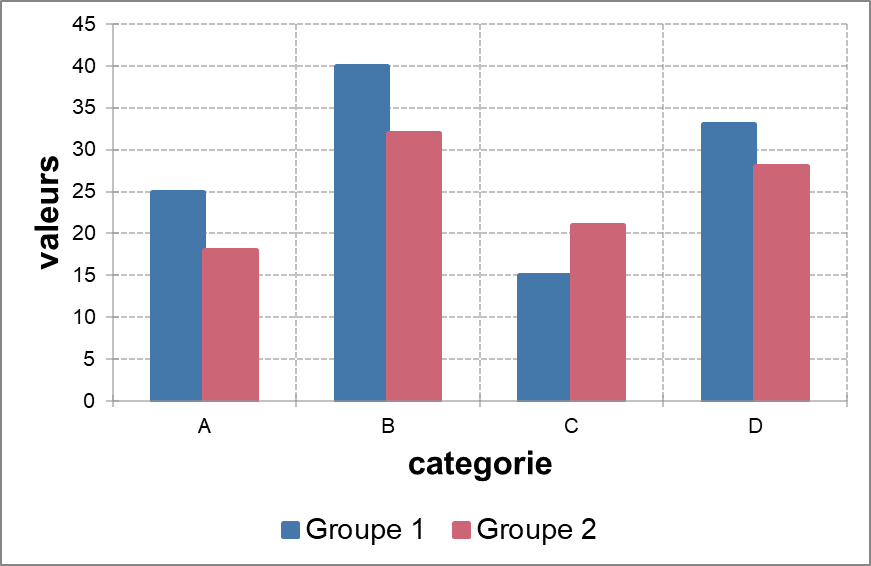
\includegraphics[keepaspectratio]{images/clipboard-1570611896.png}}

\pandocbounded{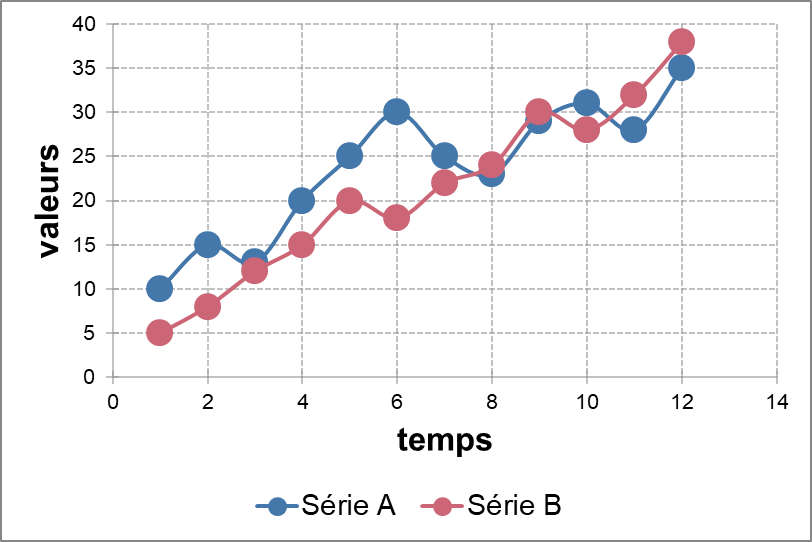
\includegraphics[keepaspectratio]{images/clipboard-3660276528.png}}

\pandocbounded{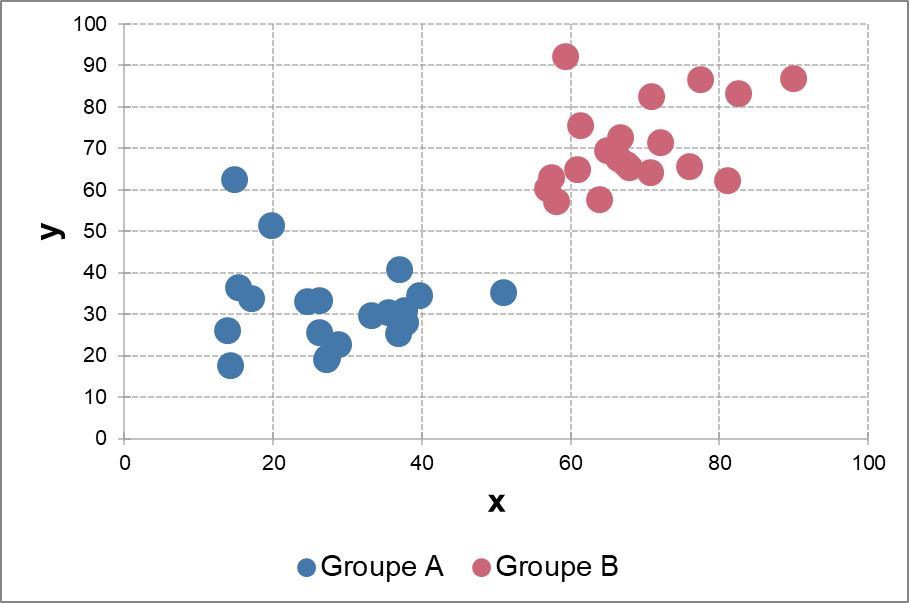
\includegraphics[keepaspectratio]{images/clipboard-1944880102.png}}

\subsection{2. Faire des graphiques éditables avec
rvg}\label{faire-des-graphiques-uxe9ditables-avec-rvg}

Le package \textbf{\texttt{rvg}} est un outil très utile lorsqu'on
souhaite \textbf{transformer des graphiques R en objets modifiables
directement dans PowerPoint}.

Plus précisément, il permet de \textbf{convertir des graphiques créés
avec \texttt{ggplot2} ou la base R (\texttt{plot()}) en objets
vectoriels}, appelés \emph{DrawingML}, qui peuvent être \textbf{édités
directement dans PowerPoint}. Cela signifie que l'on peut
\textbf{changer les couleurs, les titres, les polices ou même supprimer
des éléments}, sans avoir à retourner dans R.

Toutefois, cette fonctionnalité n'est \textbf{possible que pour les
sorties PowerPoint (\texttt{.pptx})}, et \textbf{pas directement pour
Word}. C'est une limite du format \texttt{.docx} qui ne gère pas les
objets vectoriels de la même façon.

\textbf{Mais il existe une astuce} : on peut générer les graphiques avec
\texttt{rvg} dans un document PowerPoint, puis \textbf{les copier-coller
dans Word}. Cela demande un peu de gymnastique, mais \textbf{le résultat
en vaut la peine}

\begin{Shaded}
\begin{Highlighting}[]
\FunctionTok{library}\NormalTok{(ggplot2)}

\CommentTok{\# Données d\textquotesingle{}exemple}
\NormalTok{coffee\_preferences }\OtherTok{\textless{}{-}} \FunctionTok{data.frame}\NormalTok{(}
  \AttributeTok{type =} \FunctionTok{c}\NormalTok{(}\StringTok{"Espresso"}\NormalTok{, }\StringTok{"Cappuccino"}\NormalTok{, }\StringTok{"Café filtre"}\NormalTok{, }\StringTok{"Latte"}\NormalTok{, }\StringTok{"Mocha"}\NormalTok{, }\StringTok{"Café glacé"}\NormalTok{),}
  \AttributeTok{popularite =} \FunctionTok{c}\NormalTok{(}\DecValTok{35}\NormalTok{, }\DecValTok{25}\NormalTok{, }\DecValTok{20}\NormalTok{, }\DecValTok{15}\NormalTok{, }\DecValTok{10}\NormalTok{, }\DecValTok{30}\NormalTok{)}
\NormalTok{)}

\CommentTok{\# Graphique circulaire}
\NormalTok{plot }\OtherTok{\textless{}{-}} \FunctionTok{ggplot}\NormalTok{(coffee\_preferences, }\FunctionTok{aes}\NormalTok{(}\AttributeTok{x =} \StringTok{""}\NormalTok{, }\AttributeTok{y =}\NormalTok{ popularite, }\AttributeTok{fill =}\NormalTok{ type)) }\SpecialCharTok{+}
  \FunctionTok{geom\_bar}\NormalTok{(}\AttributeTok{stat =} \StringTok{"identity"}\NormalTok{, }\AttributeTok{width =} \DecValTok{1}\NormalTok{, }\AttributeTok{color =} \StringTok{"white"}\NormalTok{) }\SpecialCharTok{+}
  \FunctionTok{coord\_polar}\NormalTok{(}\StringTok{"y"}\NormalTok{, }\AttributeTok{start =} \DecValTok{0}\NormalTok{) }\SpecialCharTok{+}
  \FunctionTok{theme\_void}\NormalTok{() }\SpecialCharTok{+}
  \FunctionTok{labs}\NormalTok{(}
    \AttributeTok{fill =} \StringTok{"Type de café"}\NormalTok{,}
    \AttributeTok{title =} \StringTok{"Popularité des types de café"}
\NormalTok{  ) }\SpecialCharTok{+}
  \FunctionTok{scale\_fill\_manual}\NormalTok{(}\AttributeTok{values =} \FunctionTok{c}\NormalTok{(}\StringTok{"\#8B4513"}\NormalTok{, }\StringTok{"\#A0522D"}\NormalTok{, }\StringTok{"\#CD853F"}\NormalTok{, }\StringTok{"\#D2B48C"}\NormalTok{, }\StringTok{"\#DEB887"}\NormalTok{, }\StringTok{"\#F5DEB3"}\NormalTok{)) }\SpecialCharTok{+}
  \FunctionTok{theme}\NormalTok{(}
    \AttributeTok{plot.title =} \FunctionTok{element\_text}\NormalTok{(}\AttributeTok{hjust =} \FloatTok{0.5}\NormalTok{, }\AttributeTok{color =} \StringTok{"\#654321"}\NormalTok{, }\AttributeTok{face =} \StringTok{"bold"}\NormalTok{),}
    \AttributeTok{legend.title =} \FunctionTok{element\_text}\NormalTok{(}\AttributeTok{color =} \StringTok{"\#654321"}\NormalTok{)}
\NormalTok{  )}
\NormalTok{rvg}\SpecialCharTok{::}\FunctionTok{dml}\NormalTok{(}\AttributeTok{ggobj =}\NormalTok{ plot) }\CommentTok{\# pour le transformer en graphique éditable}
\end{Highlighting}
\end{Shaded}

\pandocbounded{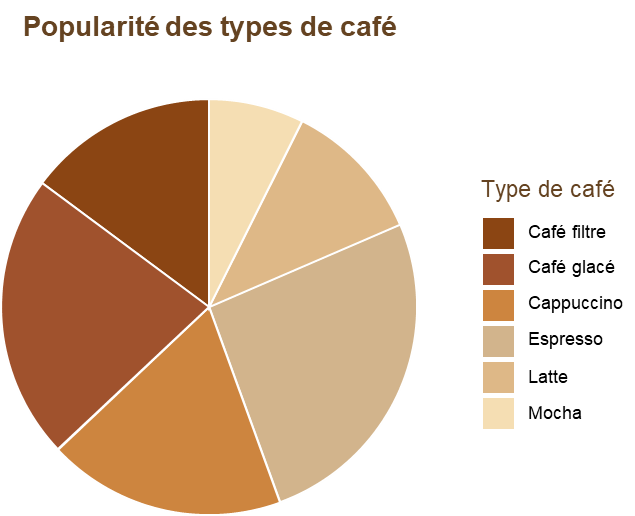
\includegraphics[keepaspectratio]{images/clipboard-3004425770.png}}

\subsection{3. Comparaison et cas
d'utilisation}\label{comparaison-et-cas-dutilisation}

Les deux approches ont leurs avantages :

\textbf{Avantages de mschart :}

\begin{itemize}
\tightlist
\item
  Graphiques modifiables directement dans Word
\item
  Contient les données sources (mise à jour possible)
\item
  Intégration parfaite avec l'esthétique Office
\item
  Idéal pour les documents destinés à la modification
\item
  Interface familière pour les utilisateurs Office
\end{itemize}

\textbf{Avantages de ggplot2 avec rvg :}

\begin{itemize}
\tightlist
\item
  Personnalisation extrêmement poussée
\item
  Grande variété de types de graphiques
\item
  Contrôle précis de tous les éléments visuels
\end{itemize}

Le choix entre ces deux approches dépend principalement de l'utilisation
prévue du document final et des besoins de personnalisation.

\newpage

\section{VI. Navigation et référencement dans le
document}\label{vi.-navigation-et-ruxe9fuxe9rencement-dans-le-document}

Un document professionnel nécessite des éléments de navigation
efficaces. Officedown nous donne des solutions assez pratiques à cet
effet.

\subsection{1. Table des matières
personnalisée}\label{table-des-matiuxe8res-personnalisuxe9e}

La table des matières peut être insérée précisément où vous le souhaitez
avec un contrôle sur sa profondeur :

\begin{Shaded}
\begin{Highlighting}[]
\NormalTok{\textless{}!{-}{-}{-}BLOCK\_TOC:depth=3{-}{-}{-}\textgreater{}}
\end{Highlighting}
\end{Shaded}

Cette instruction permet d'insérer une table des matières qui inclura
les titres jusqu'au niveau 3 (chapitres, sections, et sous-sections).

\subsection{2. Liste des figures}\label{liste-des-figures}

Pour insérer la liste des graphiques, on écrit la commande suivante :

\begin{Shaded}
\begin{Highlighting}[]
\NormalTok{\textless{}!{-}{-}{-}BLOCK\_TOC\{seq\_id: \textquotesingle{}fig\textquotesingle{}\}{-}{-}{-}\textgreater{}}
\end{Highlighting}
\end{Shaded}

Il suffit juste d'ajouter dans les infos concernant le chunk,
\texttt{fig.cap=\ "Nom\ du\ tableau"} comme dans l'exemple suivant :

\begin{Shaded}
\begin{Highlighting}[]

\NormalTok{\textasciigrave{}\textasciigrave{}\textasciigrave{} r}
\NormalTok{Mettre ici le code pour le graphique}
\end{Highlighting}
\end{Shaded}

\begin{verbatim}

## 3. Liste des tableaux

Pour générer la liste des tableaux, il ne suffit pas de mettre `tab.cap`, il faut définir le caption du graphique directement avec le package choisi pour tracer le graphique.
- Pour le package flextable, il faut utiliser la fonction `set_caption()` avec les paramètres `caption` et `autonum` comme dans l'exemple suivant : 


``` r
library(flextable)

donnees <- data.frame(
  Variable = c("Age", "Taille", "Poids"),
  Moyenne = c(34.2, 172.5, 68.7),
  Ecart_type = c(8.4, 10.2, 12.3)
)

# flextable utilise set_caption() pour définir la légende
flextable(donnees) %>%
  set_caption(
    caption = "Consommation, production et échanges de café par pays (kg par habitant)",
    autonum = run_autonum(seq_id = "tab", bkm = "tab_produits") # Pour la numérotation automatique et le signet
  )) %>%
  theme_booktabs() %>%
  autofit()
\end{verbatim}

\begin{itemize}
\tightlist
\item
  Pour le package \texttt{gtsummary()}, c'est la fonction
  \texttt{modify\_caption()} Cette instruction insère une liste de tous
  les tableaux du document.
\end{itemize}

\begin{Shaded}
\begin{Highlighting}[]
\NormalTok{\textless{}!{-}{-}{-}BLOCK\_TOC\{seq\_id: \textquotesingle{}tab\textquotesingle{}\}{-}{-}{-}\textgreater{}}
\end{Highlighting}
\end{Shaded}

Cette instruction insère une liste de tous les tableaux du document.

\subsection{4. Signets et hyperliens}\label{signets-et-hyperliens}

officedown permet également de créer des signets et des hyperliens
internes :

\subsubsection{Création d'un signet dans un
titre}\label{cruxe9ation-dun-signet-dans-un-titre}

\begin{Shaded}
\begin{Highlighting}[]
\NormalTok{Introduction à la méthodologie \{\#section\_methodo\}}
\end{Highlighting}
\end{Shaded}

Cela génère automatiquement un \textbf{signet Word} appelé
\texttt{section\_methodo}.

\subsubsection{Faire un lien vers ce
signet}\label{faire-un-lien-vers-ce-signet}

\begin{Shaded}
\begin{Highlighting}[]
\NormalTok{Pour plus de détails, voir la [section méthodologie](\#section\_methodo).}
\end{Highlighting}
\end{Shaded}

Ce lien fonctionne comme un \textbf{hyperlien interne} dans le document
Word final.

\section{VII. Notes de bas de page}\label{vii.-notes-de-bas-de-page}

Les notes de bas de page sont essentielles pour fournir des informations
supplémentaires sans perturber le flux principal du texte. En RMarkdown
avec officedown, elles sont faciles à implémenter :

\begin{itemize}
\tightlist
\item
  La syntaxe est la suivante :
\end{itemize}

\begin{Shaded}
\begin{Highlighting}[]
\NormalTok{L\textquotesingle{}analyse a révélé une corrélation significative entre les variables[\^{}1].}

\NormalTok{[\^{}1]: Le seuil de significativité a été fixé à p \textbackslash{}\textless{} 0,05 pour toutes les analyses.}
\end{Highlighting}
\end{Shaded}

\begin{itemize}
\tightlist
\item
  Le résultat est le suivant :
\end{itemize}

L'analyse statistique a révélé une corrélation significative\footnote{Le
  seuil de significativité a été fixé à p \textless{} 0,05 pour toutes
  les analyses.}.

Ces notes de bas de page sont automatiquement numérotées et formatées
selon les conventions typographiques standards.

\newpage

\section{VIII. Utilisation de templates Word
existants}\label{viii.-utilisation-de-templates-word-existants}

Pour une intégration parfaite avec les normes institutionnelles, il est
souvent judicieux d'utiliser un template Word existant.

Les étapes à suivre sont les suivantes

\begin{enumerate}
\def\labelenumi{\arabic{enumi}.}
\item
  Creer un template Word s'il n'existe pas déjà
\item
  L'utiliser dans le R markdown en insérant dans le YAML avec
  reference\_docx comme ceci :
\end{enumerate}

\begin{Shaded}
\begin{Highlighting}[]
\FunctionTok{output}\KeywordTok{:}\AttributeTok{ }
\AttributeTok{  officedown:}\FunctionTok{:rdocx\_document}\KeywordTok{:}
\AttributeTok{    }\FunctionTok{reference\_docx}\KeywordTok{:}\AttributeTok{ }\StringTok{"template\_word.docx"}
\end{Highlighting}
\end{Shaded}

Cette approche permet d'hériter de tous les styles, en-têtes, pieds de
page et autres éléments de mise en page prédéfinis dans le template.

\subsection{Comment les styles RMarkdown se lient aux styles
Word}\label{comment-les-styles-rmarkdown-se-lient-aux-styles-word}

\begin{longtable}[]{@{}ll@{}}
\toprule\noalign{}
Élément RMarkdown & Style Word attendu \\
\midrule\noalign{}
\endhead
\bottomrule\noalign{}
\endlastfoot
\texttt{\#\ Mon\ titre} & Heading 1 \\
\texttt{\#\#\ Sous-titre} & Heading 2 \\
Texte normal & Normal \\
Tableaux \texttt{flextable} & Table \\
Graphiques \texttt{ggplot} (\texttt{rvg}) & Figure \\
Titre du document & Title \\
\end{longtable}

Si ces styles sont bien définis dans le modèle Word, le rendu final sera
parfaitement formaté.

\subsection{Qu'est ce que le document va hériter du
template}\label{quest-ce-que-le-document-va-huxe9riter-du-template}

\begin{longtable}[]{@{}
  >{\raggedright\arraybackslash}p{(\linewidth - 2\tabcolsep) * \real{0.3889}}
  >{\raggedright\arraybackslash}p{(\linewidth - 2\tabcolsep) * \real{0.6111}}@{}}
\toprule\noalign{}
\begin{minipage}[b]{\linewidth}\raggedright
Élément hérité
\end{minipage} & \begin{minipage}[b]{\linewidth}\raggedright
Description
\end{minipage} \\
\midrule\noalign{}
\endhead
\bottomrule\noalign{}
\endlastfoot
\textbf{Styles de paragraphe} (\texttt{Normal}, \texttt{Heading\ 1},
etc.) & Le texte, les titres, les sous-titres, les légendes suivront les
styles Word définis dans le template \\
\textbf{Police} (type, taille) & Par défaut, la police du texte, des
titres, des tableaux est celle du modèle Word \\
\textbf{Couleurs du texte et des titres} & Si tes titres ou paragraphes
ont une couleur dans le template, ton document les utilisera \\
\textbf{Interligne et espacement} & Gérés dans les styles Word → ton R
Markdown va s'adapter automatiquement \\
\textbf{Mise en page globale} (marges, orientation) & Le document
respecte les marges, en-têtes et pieds de page du modèle \\
\textbf{Styles de tableaux} (\texttt{Table}) & Les tableaux générés avec
\texttt{flextable} peuvent utiliser les styles Word définis (bordures,
couleurs\ldots) \\
\textbf{Style d'image ou de légende} (\texttt{Figure}) & Les images et
graphiques peuvent hériter d'un style spécifique défini dans Word \\
\textbf{En-têtes et pieds de page} & Logo, date, pagination : tout ce
qui est dans l'en-tête/pied du modèle est repris \\
\end{longtable}

\section{Conclusion}\label{conclusion}

\subsection{Avantages de l'approche
officedown}\label{avantages-de-lapproche-officedown}

L'utilisation de RMarkdown avec le package officedown pour la génération
de rapports Word présente plusieurs avantages significatifs :

\begin{enumerate}
\def\labelenumi{\arabic{enumi}.}
\item
  \textbf{Reproductibilité analytique} : Le code R et son résultat sont
  liés, garantissant que les tableaux et graphiques correspondent aux
  analyses effectuées.
\item
  \textbf{Efficacité et gain de temps} : Les modifications des données
  ou des analyses sont propagées automatiquement dans l'ensemble du
  document, éliminant le besoin de mettre à jour manuellement les
  résultats.
\item
  \textbf{Cohérence visuelle} : Les styles définis peuvent être
  réutilisés systématiquement, assurant une présentation cohérente tout
  au long du document.
\item
  \textbf{Flexibilité de format} : Un même document source peut générer
  différents formats de sortie (Word, PDF, HTML) selon les besoins.
\item
  \textbf{Contrôle avancé} : officedown offre un niveau de contrôle sur
  la mise en page et la structure du document qui dépasse les capacités
  de RMarkdown standard.
\end{enumerate}

\subsection{Limites et solutions
alternatives}\label{limites-et-solutions-alternatives}

Malgré ses nombreux avantages, cette approche présente quelques
limitations :

\begin{enumerate}
\def\labelenumi{\arabic{enumi}.}
\item
  \textbf{Courbe d'apprentissage} : La maîtrise de RMarkdown, officedown
  et des packages associés nécessite un investissement initial en temps
  et en formation.
\item
  \textbf{Éléments extérieurs au contenu} : Certains éléments comme les
  en-têtes et pieds de page complexes restent plus faciles à gérer
  directement dans Word.
\item
  \textbf{Contrôle pixel-parfait} : Pour des mises en page très
  spécifiques, l'édition directe dans Word après génération peut rester
  nécessaire.
\end{enumerate}

\end{document}
